% Suggested figure environments; add \usepackage{graphicx} and \usepackage{booktabs} in preamble.
% Paths assume compilation from project root; adapt if thesis is elsewhere.
% Figure 10 should REPLACE Figures 8 and 9, not accompany both.


% ---------------- Chapter section 3.3 ----------------
\begin{figure}[tbp]
    \centering
    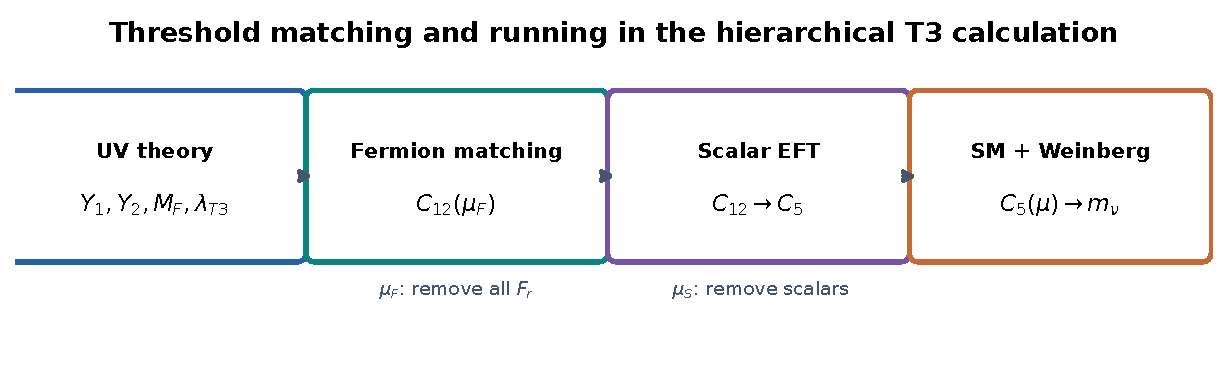
\includegraphics[width=0.87\textwidth]{Reports/output/thesis_assets/figures/fig01_t3_effective_theory_flow.pdf}
    \caption{Hierarchical matching and evolution in the T3 calculation, including simultaneous removal of the heavy fermions at $\mu_F$, generation of $C_{12}$, fixed-order $C_{12}\rightarrow C_5$ transport in the scalar-only EFT, and final SM+Weinberg evolution. Schematic, not a numerical trajectory.}
    \label{fig:t3-eft-flow}
\end{figure}
% Priority: CORE -- Effective theory sequence (schematic)


% ---------------- Chapter section 3.5 ----------------
\begin{figure}[tbp]
    \centering
    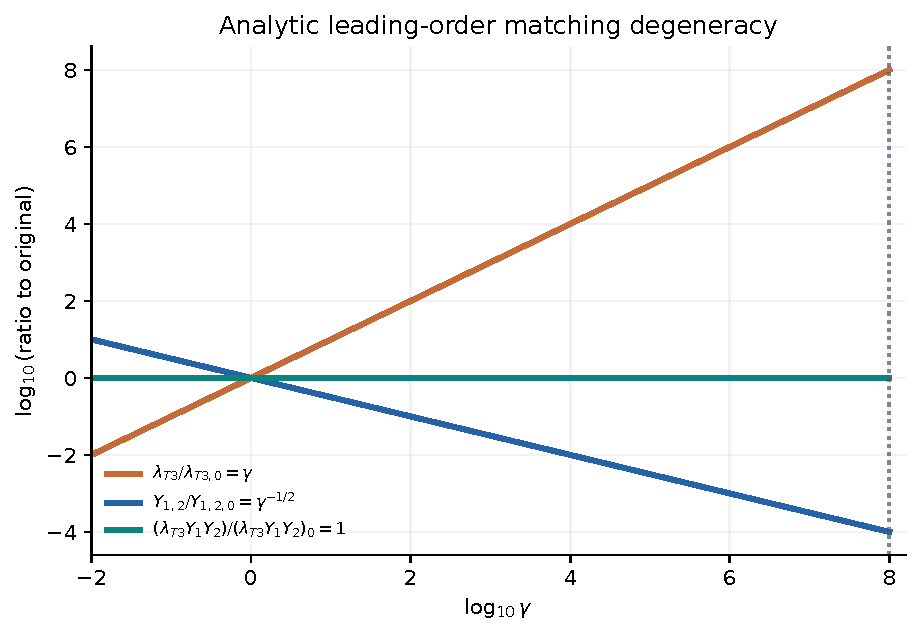
\includegraphics[width=0.87\textwidth]{Reports/output/thesis_assets/figures/fig02_analytic_coupling_scaling.pdf}
    \caption{Algebraic scaling direction $\lambda_{T3}\rightarrow\gamma\lambda_{T3}$, $Y_{1,2}\rightarrow\gamma^{-1/2}Y_{1,2}$ that preserves the leading bilinear matching factor $\lambda_{T3}Y_1Y_2$. This does not include RGE evolution or numerical parameter constraints.}
    \label{fig:t3-scaling}
\end{figure}
% Priority: OPTIONAL -- Leading matching rescaling (analytic; NOT an RGE scan)


% ---------------- Chapter section 5.1 ----------------
\begin{figure}[tbp]
    \centering
    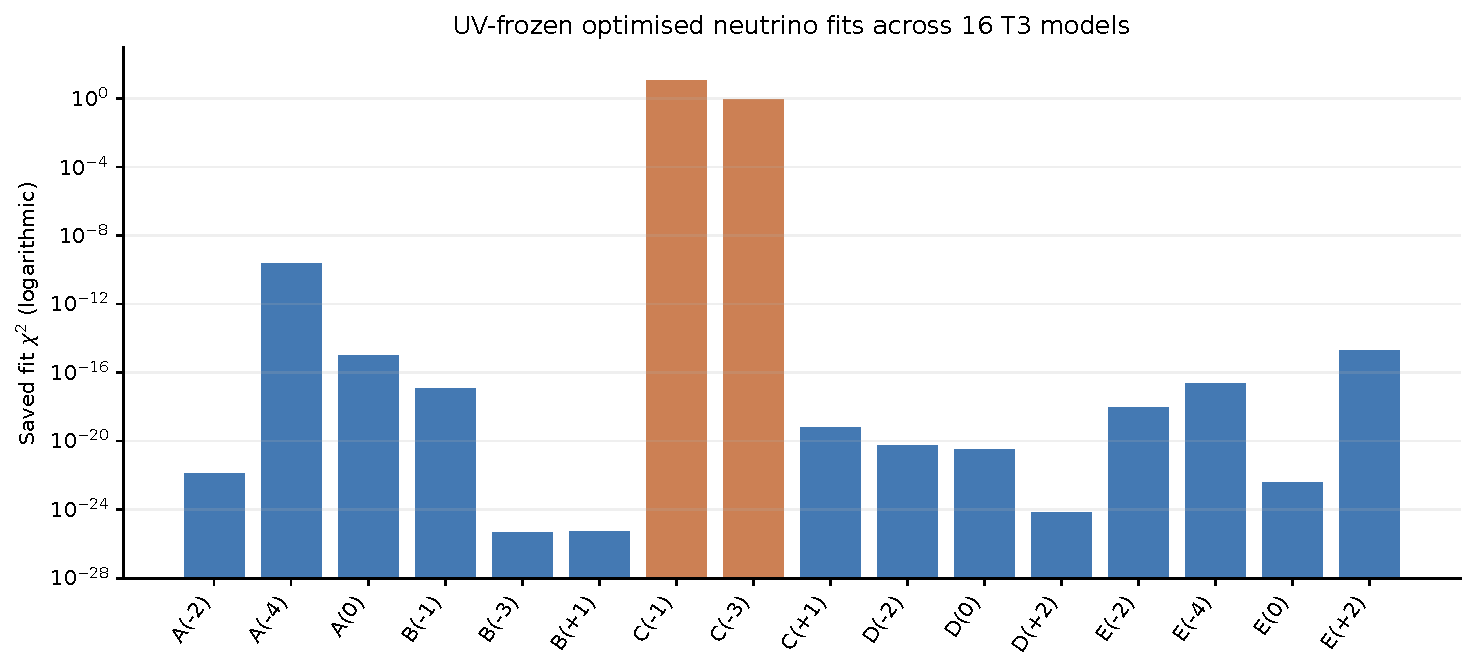
\includegraphics[width=0.87\textwidth]{Reports/output/thesis_assets/figures/fig03_optimised_fit_quality_16_models.pdf}
    \caption{Saved optimised fit objectives for sixteen T3 models with frozen UV running at $\lambda_{T3}=5\times10^{-9}$. The bars are fit $\chi^2$ values; they are not likelihood-ratio comparisons or model preferences.}
    \label{fig:t3-fits}
\end{figure}
% Priority: OPTIONAL -- Sixteen saved fitted objectives (fit quality, not model evidence)


% ---------------- Chapter section 5.3 ----------------
\begin{figure}[tbp]
    \centering
    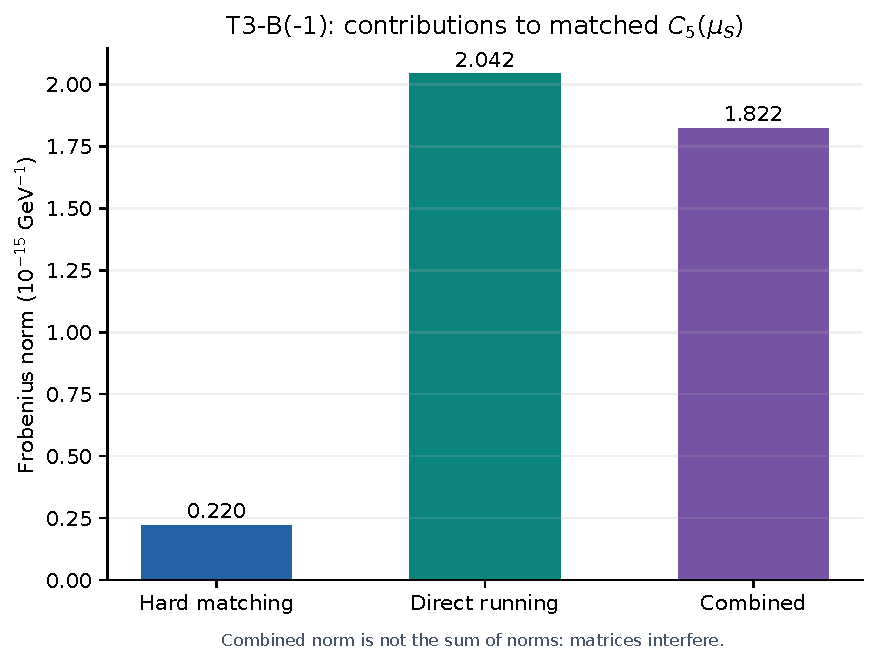
\includegraphics[width=0.87\textwidth]{Reports/output/thesis_assets/figures/fig07_t3b_c5_threshold_components.pdf}
    \caption{Frobenius norms of hard matching, direct $C_{12}\rightarrow C_5$ running and their combined scalar-threshold coefficient for the UV-frozen T3-B(-1) benchmark. The combined norm is not the sum of the individual norms because the matrices interfere.}
    \label{fig:t3-c5-contributions}
\end{figure}
% Priority: CORE -- Hard versus direct contribution to final C5


% ---------------- Chapter section 5.6.1 ----------------
\begin{figure}[tbp]
    \centering
    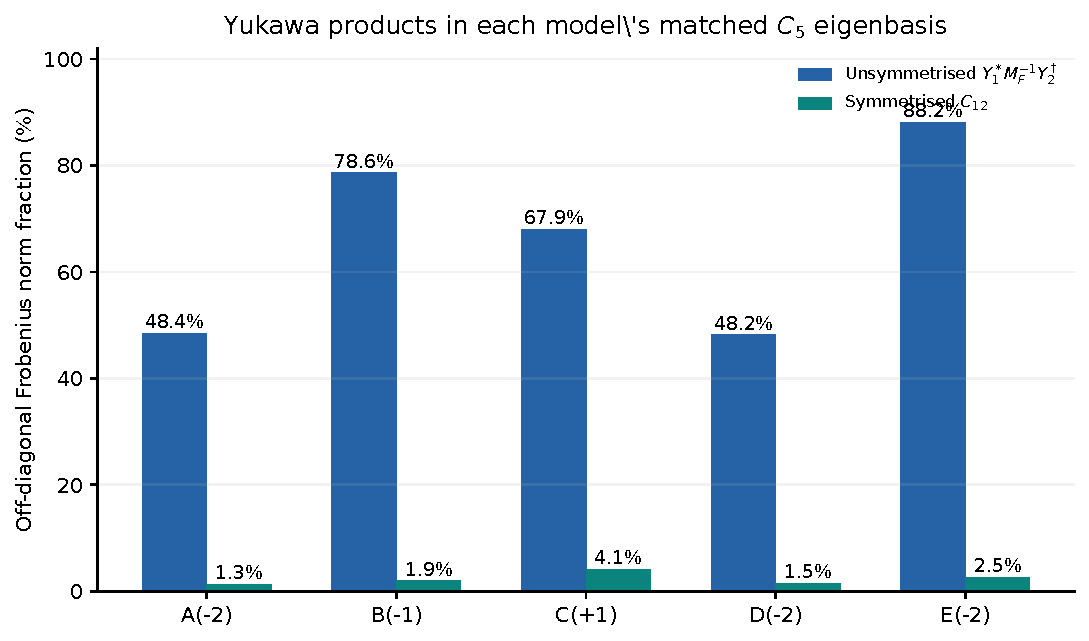
\includegraphics[width=0.87\textwidth]{Reports/output/thesis_assets/figures/fig04_five_class_flavour_alignment.pdf}
    \caption{Off-diagonal norm fractions of the unsymmetrised mass-weighted Yukawa product and the symmetrised $C_{12}$ in the eigenbasis of each model's matched $C_5$. Five fitted UV-frozen class representatives. Symmetrisation does not imply diagonality in general.}
    \label{fig:t3-flavour-five-classes}
\end{figure}
% Priority: CORE -- Unsymmetrised versus symmetrised flavour alignment (five classes)


% ---------------- Chapter section 5.6.2 ----------------
\begin{figure}[tbp]
    \centering
    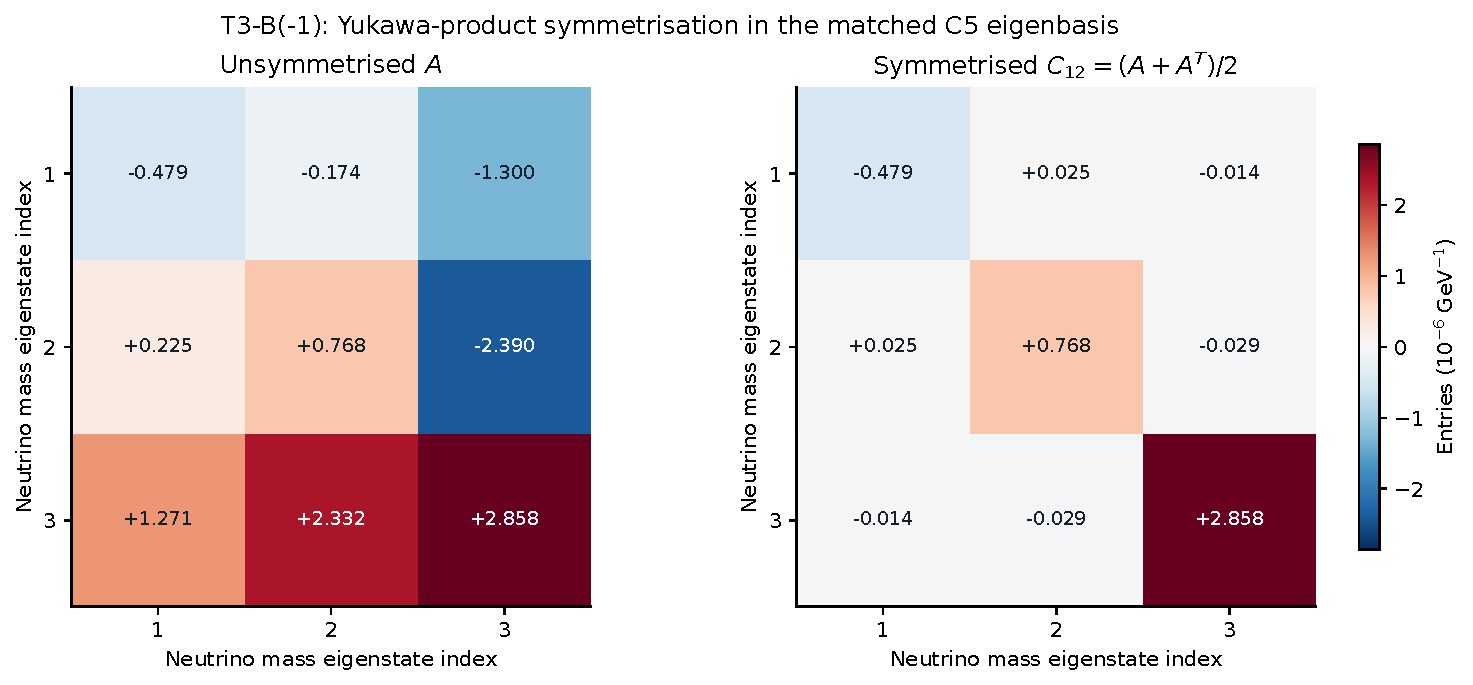
\includegraphics[width=0.87\textwidth]{Reports/output/thesis_assets/figures/fig05_t3b_yukawa_product_matrices.pdf}
    \caption{T3-B(-1) unsymmetrised Yukawa product and its symmetric part $C_{12}$ expressed in the eigenbasis of the complete matched $C_5$, in $10^{-6}\,\mathrm{GeV}^{-1}$.}
    \label{fig:t3-yukawa-heatmap}
\end{figure}
% Priority: OPTIONAL -- T3-B matrix example before/after symmetrisation


% ---------------- Chapter section 5.6.3 ----------------
\begin{figure}[tbp]
    \centering
    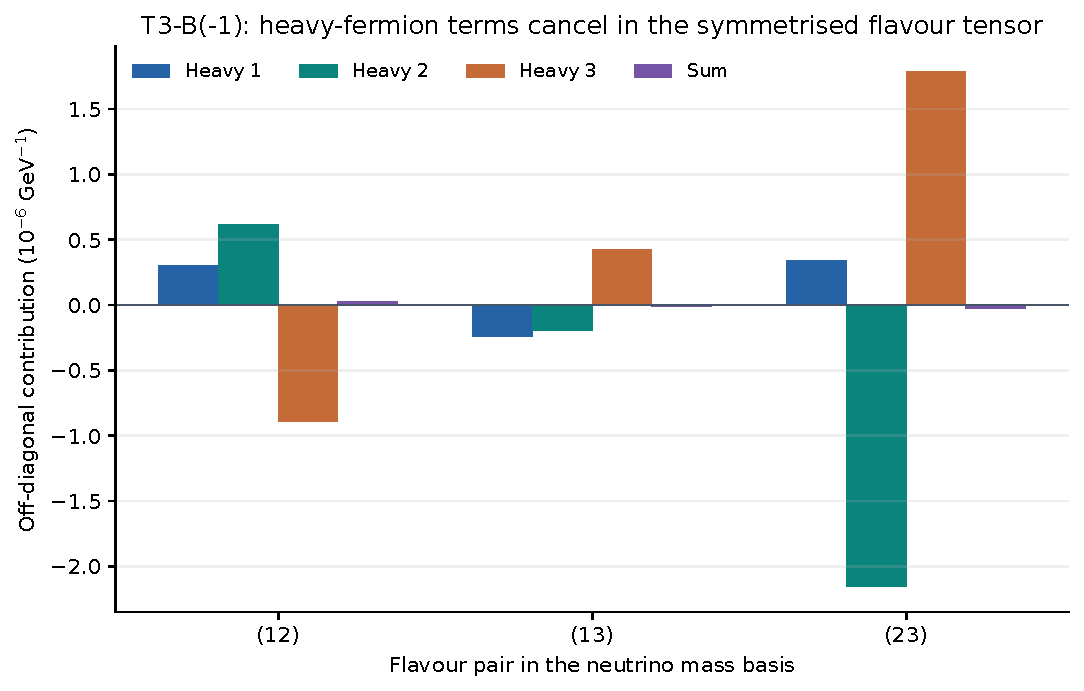
\includegraphics[width=0.87\textwidth]{Reports/output/thesis_assets/figures/fig06_t3b_heavy_state_cancellations.pdf}
    \caption{Contributions of the three heavy fermions to the off-diagonal components of the fitted T3-B(-1) $C_{12}$ matrix in the matched-$C_5$ eigenbasis. The small sums arise from cancellations between large individual terms.}
    \label{fig:t3-heavy-cancellation}
\end{figure}
% Priority: CORE -- Cancellation by heavy-fermion state


% ---------------- Chapter section 5.6.4 ----------------
\begin{figure}[tbp]
    \centering
    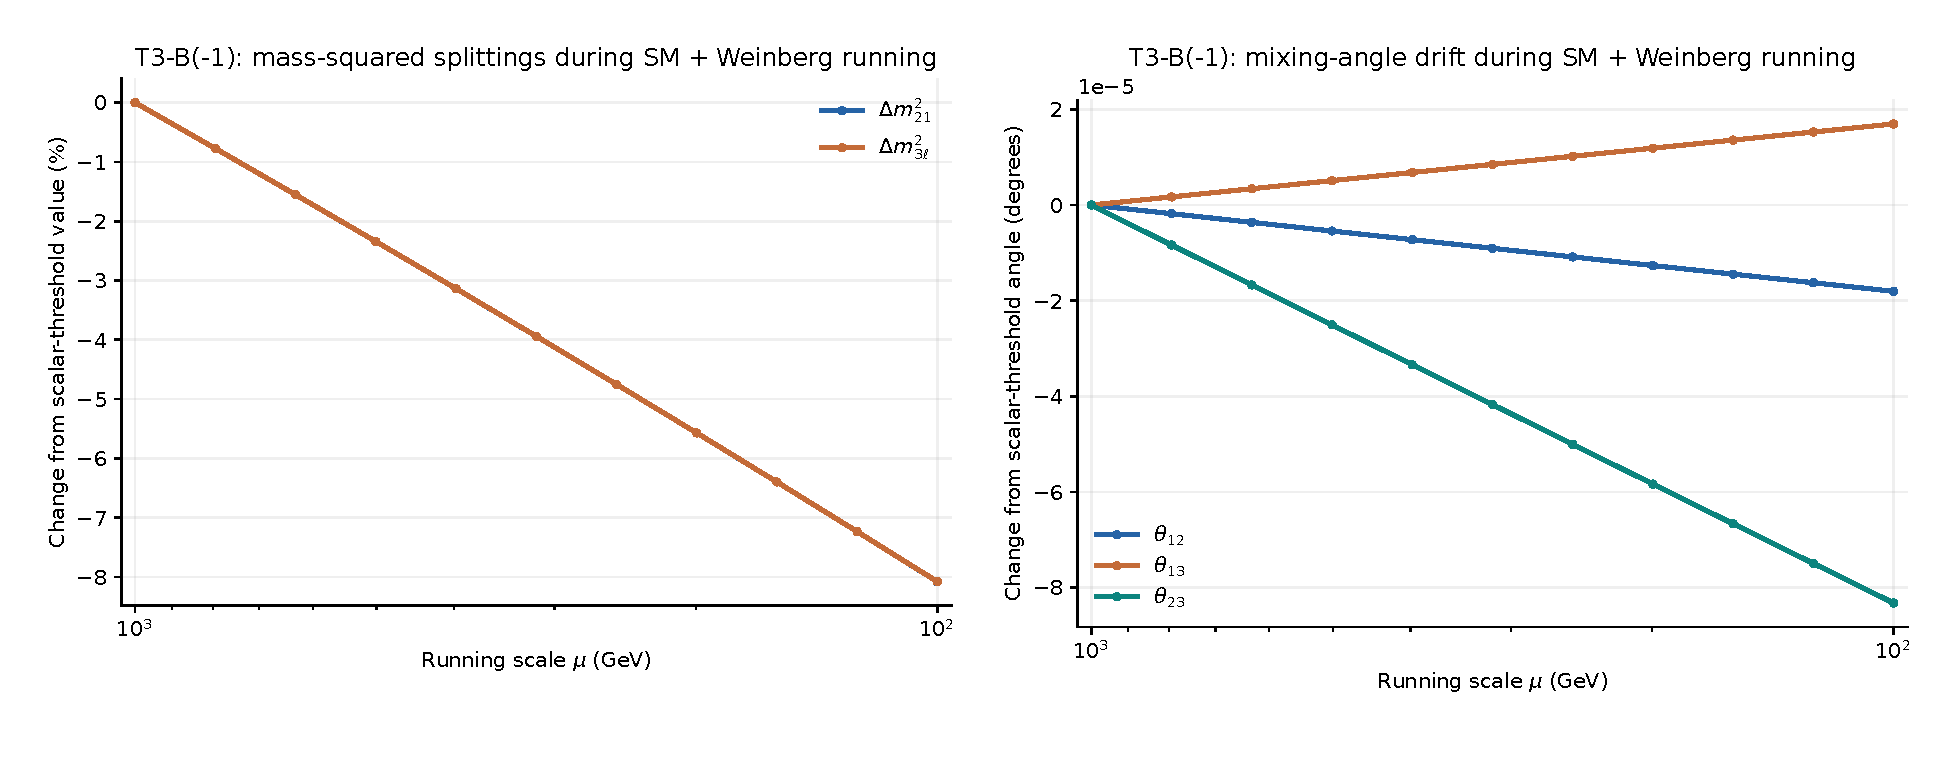
\includegraphics[width=1.0\textwidth]{Reports/output/thesis_assets/figures/fig10_mass_vs_mixing_running_combined.pdf}
    \caption{Comparison of mass-squared-splitting evolution (left) and mixing-angle drift (right) in the final SM+Weinberg EFT, from $1\,\mathrm{TeV}$ to $100\,\mathrm{GeV}$, for the fitted UV-frozen T3-B(-1) benchmark at $\lambda_{T3}=5\times10^{-9}$. Both splittings change by approximately $8.08\%$, while angle changes are smaller than $10^{-4}$ degrees. These panels do not show scalar-only EFT PMNS running.}
    \label{fig:t3-masses-versus-mixing}
\end{figure}
% Priority: CORE -- Two-panel mass-squared versus mixing-angle running


% Example: include the selected numeric tables (booktabs required).
% \begin{table}[htbp]
\centering
\caption{Hard, direct-running, and combined matched $C_5$ for the UV-frozen T3-B(-1) benchmark.}
\label{tab:t3-c5-decomposition}
\begin{tabular}{lrr}
\toprule
Component & $\|C_5\|_F$ (GeV$^{-1}$) & Off-diagonal (\%) \\
\midrule
Hard & $2.204\times10^{-16}$ & $1.943$ \\
Direct running & $2.042\times10^{-15}$ & $0.210$ \\
Combined & $1.822\times10^{-15}$ & $0.000$ \\
\bottomrule
\end{tabular}
\end{table}

% \begin{table}[htbp]
\centering
\caption{Saved T3-B(-1) Weinberg-stage predictions at $\mu_S=1$ TeV and $\mu_{\rm low}=100$ GeV. Angles are presented as $\sin^2\theta_{ij}$.}
\label{tab:t3-weinberg-endpoints}
\begin{tabular}{lrrr}
\toprule
Observable & 1 TeV & 100 GeV & Change (\%) \\
\midrule
delta\_m21\_sq\_ev2 & $8.19932\times10^{-5}$ & $7.537\times10^{-5}$ & $-8.0778$ \\
delta\_m3l\_sq\_ev2 & $2.73165\times10^{-3}$ & $2.511\times10^{-3}$ & $-8.0776$ \\
sin2\_theta12 & $0.308800$ & $0.308800$ & $-0.0001$ \\
sin2\_theta13 & $0.022480$ & $0.022480$ & $+0.0004$ \\
sin2\_theta23 & $0.470001$ & $0.470000$ & $-0.0003$ \\
\bottomrule
\end{tabular}
\end{table}

